\documentclass[]{article}

\usepackage[utf8]{inputenc}
\usepackage[english]{babel}
\usepackage{amsthm}
\usepackage{amssymb}
\usepackage{amsmath}
\usepackage{tikz}
\usetikzlibrary{arrows}

\newcommand{\approxq}{\stackrel{?}{\approx}}
\newcommand{\moreGeneral}{\lesssim^X_E}
\newcommand{\eqClass}{\sim^X_E}

%opening
\title{}
\author{}
\newtheorem{theorem}{Theorem}[section]
\newtheorem{lemma}[theorem]{Lemma}
\theoremstyle{definition}
\newtheorem{definition}[theorem]{Definition}

\begin{document}
	\tableofcontents \newpage
	\section{Equational Unification}
In the following let $E$ be a set of identities of the form $\left\lbrace  e_1\approx f_1,\dots,e_n\approx f_n \right\rbrace$. Furthermore let $\mathcal{S}ig(E)$ denote the set of all function symbols occurring in $E$. Let $\Sigma$ be a finite set of function symbols and a superset of $\mathcal{S}ig(E)$.
\begin{definition}
An \textbf{$E$-unification Problem} over $\Sigma$ is a finite set $S$ of the form $S=\left\lbrace s_1\approxq_{E} t_1,\dots,s_n\approxq_{E} t_n\right\rbrace $ with $s_1,\dots,s_n,t_1,\dots,t_n \in T(\Sigma,V)$, $V$ being a countable set of Variables.\\
A substitution $\sigma$ is an \textbf{$E$-unifier} of $S$ iff $ \sigma(s_i)\approx_E \sigma(t_i)$ for all $1\leq i \leq n$.
The set of all $E$-unifiers of $S$ is denoted by $\mathcal{U}_E(S)$. $S$ is \textbf{$E$-unifiable} iff $\mathcal{U}_E(S)\neq \emptyset$.
\end{definition}
\begin{definition}
Let $S$ be an $E$-unification problem over $\Sigma$.
\begin{itemize}
\item $S$ is an \textbf{elementary} $E$-unification problem iff $\mathcal{S}ig(E)=\Sigma$.
\item $S$ is an $E$-unification problem \textbf{with constants} iff $\Sigma-\mathcal{S}ig(E)\subseteq\Sigma^{(0)}$ and $\mathcal{S}ig(E)\subset\Sigma$
\item $S$ is an \textbf{general} $E$-unification problem iff $\Sigma-\mathcal{S}ig(E)$ contains an at least unary function symbol.
\end{itemize}
\end{definition}
%To see why this classification makes sense lets consider the set 
%...
One $most\ general\ unifier$ does not always suffice to represent $\mathcal{U}_E(S)$. In this case we need a $minimal\ complete\ set\ of\ unifiers$ but to define this set we first need an order on substitutions.
\begin{definition}
Let $X$ be a set of variables. A substitution $\sigma$ is \textbf{more general} modulo $\approx_E$ than a substitution $\sigma'$ on $X$ iff there is a substitution $\delta$ such that $\delta(\sigma(x))\approx_E\sigma'(x)$ for all $x \in X$. We denote this by $\sigma\moreGeneral\sigma'$.
\end{definition}
$\moreGeneral$ is a is a quasi order since it obviously is reflexive and transitive. But why do we only demand equality modulo $\approx_E$ on $X$ and not on all Variables like we did in syntactic unification? Note that by the restriction to Variables in $X$ more substitutions are comparable with respect to $\moreGeneral$ since we do not demand equality modulo $\approx_E$ on all Variables. Lets denote the Variables occurring in an $E$-unification problem $S$ by $\mathcal{V}ar(S)$. It is easy to see that if $X=\mathcal{V}ar(S)$, $\sigma'$ is an $E$-unifier of $S$ and $\sigma\moreGeneral\sigma'$ then $\sigma$ is also an $E$-unifier of $S$. This only shows that restriction to $X$ does not do any damage but the reason it is useful is that there are $E$-unification problems $S$ for which any $minimal\ complete\ set\ of\ E$-$unifiers$ has to contain Variables not occurring in $S$. Lets consider a small example, let $\sigma:=\left\lbrace x\mapsto f(y)\right\rbrace$ be in $\mathcal{M}$ a $minimal\ complete\ set\ of\ E$-$unifiers$ of $S$ with $\mathcal{V}ar(S)=\left\lbrace x\right\rbrace$ and $\left\lbrace a\approx x\right\rbrace \notin E$. Clearly $\sigma':=\left\lbrace x\mapsto f(a)\right\rbrace$ is also an $E$-unifier of $S$ but $\sigma$ and $\sigma'$ are incomparable w.r.t. $\lesssim^{\left\lbrace x,y\right\rbrace }_E$. The substitution $\delta:=\left\lbrace y\mapsto a\right\rbrace $ does not work here since $\delta(\sigma(y))=a \not\approx_E y=\sigma'(y)$ which means there has to be another unifier $\sigma''$ in $\mathcal{M}$ with $\sigma''\lesssim^{\left\lbrace x,y\right\rbrace }_E\sigma$. But if we restrict $X$ to $\left\lbrace x\right\rbrace $ we only need that $\delta(\sigma(x))=f(a) \approx_E f(a)=\sigma'(x)$ so $\sigma\lesssim^{\left\lbrace x\right\rbrace }_E\sigma'$ holds. We see that $minimal\ complete\ sets\ of\ E$-$unifiers$ can become unnecessary large if we consider all Variables. Since we have talked about these sets a lot lets define them formally.
\begin{definition}
Let $S$ be an $E$-unification problem over $\Sigma$ and let $X:=\mathcal{V}ar(S)$. An \textbf{$E$-complete} set of $S$ is a set of substitutions $\mathcal{C}$ that satisfies the following properties.
\begin{itemize}
\item each $\sigma \in \mathcal{C}$ is an $E$-unifier of $S$
\item for all $\theta \in\mathcal{U}_E(S)$ there exists a $\sigma \in \mathcal{C}$ such that $\sigma\moreGeneral\theta$
\end{itemize}
An \textbf{$E$-minimal $E$-complete} set is an $E$-complete set  $\mathcal{M}$ that satisfies the additional property
\begin{itemize}
\item for all $\sigma,\sigma'\in\mathcal{M},\ \sigma\moreGeneral\sigma'$ implies $\sigma=\sigma'$.
\end{itemize}
The substitution $\sigma$ is a \textbf{most general $E$-unifier} (mgu) of $S$ iff $\left\lbrace \sigma\right\rbrace$ is an $E$-minimal $E$-complete set of $S$.
\end{definition}
Now let us consider an example in which an $E$-minimal $E$-complete set contains infinitely many elements. Let $A:=\left\lbrace x+(y+z)\approx (x+y)+z\right\rbrace $ be a set of identities and $S:=\left\lbrace x+a\approxq_A a+x\right\rbrace$ an $A$-unification problem over $\Sigma:=\left\lbrace +,a\right\rbrace$. For $n>0$, we define substitutions $\sigma_n$ inductively as follows:
\begin{align*}
\sigma_1&:=\left\lbrace x\mapsto a\right\rbrace\\
\sigma_{n+1}&:=\left\lbrace x\mapsto a+\sigma_n(x)\right\rbrace
\end{align*}
Since $A$ axiomatizes associativity we can omit the brackets and give an explicit definition of $\sigma_n$.
\begin{align*}
\sigma_n:=\lbrace\underbrace{a+\dots+a}_{n\times a} \rbrace
\end{align*}
Now it is easy to see that all $\sigma_n$ are $A$-unifiers of $S$.
Lets consider an arbitrary $A$-unifier $\theta$ of $S$. $\theta(x)$ has the form $\theta(x):=x_1+\dots+x_n$ where the $x_i's$ are either $a$ or a variable.
Since $\theta$ is an $A$-unifier of $S$ we have that:
\begin{align*}
&&\theta(x)+a&\approx_A a+\theta(x)\\
&& x_1+\dots+x_n+a&\approx_A a+x_1+\dots+x_n\\
&\implies x_1=a,x_n=a& a+x_2+\dots+x_{n-1}+a+a&\approx_A a+a+x_2+\dots+x_{n-1}+a\\
&\implies x_2=a,x_{n-1}=a& a+a+\dots+a+a+a&\approx_A a+a+a+\dots+a+a\\
&\hspace{10pt}\vdots&&\vdots\\
&\implies&\underbrace{a+\dots+a}_{n+1\times a}&\approx_A \underbrace{a+\dots+a}_{n+1\times a}
\end{align*}
So $\theta(x)=\sigma_n(x)$ which implies $\sigma\lesssim^{\left\lbrace x\right\rbrace }_A\theta$.
Since we picked $\theta$ arbitrarily this yields $A$-completeness of the set $\mathcal{M}:=\bigcup_{n>0}\left\lbrace  \sigma_n\right\rbrace $.
All $\sigma_n$ are distinct and map x to ground terms. Hence they are pairwise incomparable with respect to $\lesssim^{\left\lbrace x\right\rbrace }_A$. This yields $A$-minimality of $\mathcal{M}$.
We see that $E$-minimal $E$-complete sets do not need to have finite cardinality.
%equivalence class induced by <=
\begin{lemma}
Let $\mathcal{M}_1$ and $\mathcal{M}_2$ be $E$-minimal $E$-complete sets of $S$. Then there exists a bijective mapping $B:\mathcal{M}_1\mapsto\mathcal{M}_2$ such that $\sigma_1\eqClass B(\sigma_1)$ for all $\sigma_1\in\mathcal{M}_1$.
\end{lemma}
\begin{proof}
We define a mapping $B:\mathcal{M}_1\mapsto\mathcal{M}_2$ such that $B(\sigma_1)\moreGeneral\sigma_1$ for all $\sigma_1\in\mathcal{M}_1$. This is possible since $\mathcal{M}_1\subseteq\mathcal{U}_E(S)$ and $E$-completeness of $\mathcal{M}_2$ yields that for every $\sigma_1\in\mathcal{M}_1$ there exists a $\sigma_2\in\mathcal{M}_2$ such that $\sigma_2\moreGeneral\sigma_1$. We define $B':\mathcal{M}_2\mapsto\mathcal{M}_1$ in a similar way.
\begin{center}
 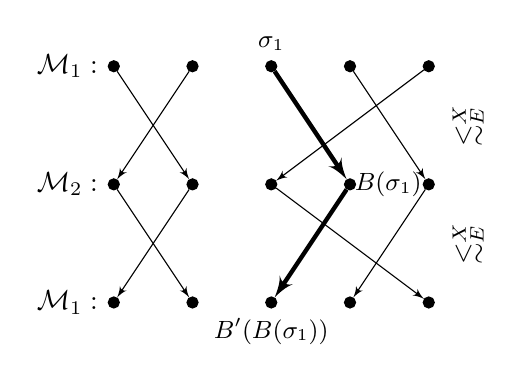
\begin{tikzpicture}
 \newcommand{\vLength}{1.5}
	\tikzset{vertex/.style = {circle,draw,fill=black,minimum size=4pt,inner sep=0pt}}
	\tikzstyle{edge} = [->,> = latex',thin]
	\tikzstyle{edgeThick} = [->,> = latex', ultra thick]
	%M_1
	\node[vertex] (00) at (0,\vLength) [label=left:$\mathcal{M}_1:$] {};
	\node[vertex] (01) at (1,\vLength) {};
	\node[vertex] (02) at (2,\vLength) [label=above:\small{$\sigma_1$}] {};
	\node[vertex] (03) at (3,\vLength) {};
	\node[vertex] (04) at (4,\vLength) {};
	%M_2
	\node[vertex] (10) at (0,0) [label=left:$\mathcal{M}_2:$] {};
	\node[vertex] (11) at (1,0) {};
	\node[vertex] (12) at (2,0) {};
	\node[vertex] (13) at (3,0) [label=right:\hspace{-4pt}\small{$B(\sigma_1)$}] {};
	\node[vertex] (14) at (4,0) {};
	%M_1 bottom
	\node[vertex] (20) at (0,-\vLength)[label=left:$\mathcal{M}_1:$] {};
	\node[vertex] (21) at (1,-\vLength) {};
	\node[vertex] (22) at (2,-\vLength) [label=below:\small{$B'(B(\sigma_1))$}] {};
	\node[vertex] (23) at (3,-\vLength) {};
	\node[vertex] (24) at (4,-\vLength) {};
	%mapping B
	\draw[edge] (00) to (11);
	\draw[edge] (01) to (10);
	\draw[edgeThick] (02) to (13);
	\draw[edge] (03) to (14);
	\draw[edge] (04) to (12);
	%mapping B'
	\draw[edge] (11) to (20);
	\draw[edge] (10) to (21);
	\draw[edgeThick] (13) to (22);
	\draw[edge] (14) to (23);
	\draw[edge] (12) to (24);
	
	\node[rotate=90] (B) at (4.5,0.5*\vLength) {$\moreGeneral$};
	\node[rotate=90] (B') at (4.5,-0.5*\vLength) {$\moreGeneral$};
\end{tikzpicture}
\end{center}
Since by definition $B'(B(\sigma_1))\moreGeneral B(\sigma_1)\moreGeneral\sigma_1$ $E$-minimality of $\mathcal{M}_1$ implies that $B'(B(\sigma_1))=\sigma_1$ for all $\sigma_1\in\mathcal{M}_1$. Symmetrically, $B(B'(\sigma_2))=\sigma_2$ for all $\sigma_2\in\mathcal{M}_2$.
\begin{center}
 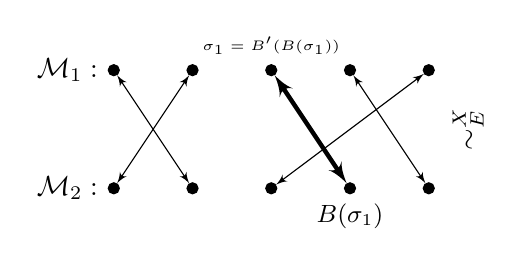
\begin{tikzpicture}
 \newcommand{\vLength}{1.5}
	\tikzset{vertex/.style = {circle,draw,fill=black,minimum size=4pt,inner sep=0pt}}
	\tikzstyle{edge} = [<->,> = latex',thin]
	\tikzstyle{edgeThick} = [<->,> = latex', ultra thick]
	%M_1
	\node[vertex] (00) at (0,\vLength) [label=left:$\mathcal{M}_1:$] {};
	\node[vertex] (01) at (1,\vLength) {};
	\node[vertex] (02) at (2,\vLength) [label=above:\tiny{$\sigma_1=B'(B(\sigma_1))$}] {};
	\node[vertex] (03) at (3,\vLength) {};
	\node[vertex] (04) at (4,\vLength) {};
	%M_2
	\node[vertex] (10) at (0,0) [label=left:$\mathcal{M}_2:$] {};
	\node[vertex] (11) at (1,0) {};
	\node[vertex] (12) at (2,0) {};
	\node[vertex] (13) at (3,0) [label=below:\small{$B(\sigma_1)$}] {};
	\node[vertex] (14) at (4,0) {};
	%mapping B
	\draw[edge] (00) to (11);
	\draw[edge] (01) to (10);
	\draw[edgeThick] (02) to (13);
	\draw[edge] (03) to (14);
	\draw[edge] (04) to (12);
	
	\node[rotate=90] (B) at (4.5,0.5*\vLength) {$\eqClass$};
\end{tikzpicture}
\end{center}
\end{proof}
\end{document}
